\section{图像分析}
\label{sec:image_analysis}

对图像进行增强、恢复、编码等处理时,输入是 图像,所要求的输出是一幅近似于输入的图像, 这是此类处理的特点。图像处理的另一主要分支 是图像分析,这类处理的输入仍然是图像,但所 要求的输出是对已知图像的描述。分析一般针对图像中的特定区域或目标。为此,传 统算法首先要进行分割(检测),有些分割运算可直接用于整个图像,而有些分割算法只适用于已被 局部分割的图像。传统图像分割是指根据灰度、彩色、空间纹理、几何形状等特征把图像划分成若干个互不相交的区域,使得这些特征在同一区域内表现出一致性或相似性,而在不同区域间表现出明显的不同。简单的说就是在一副图像中,把目标从背景中分离出来。

早期的图像分割主要是通过提取图像手工设计的特征,然后进行分割,分割出来的结果并没有语义的标注,换句话说,分割出来的东西并不知道是什么。随着计算机能力的提高,人们开始考虑获得图像的语义分割,这里的语义主要指分割出来的物体的类别。随着FCN的出现,深度学习正式进入图像语义分割领域,这里的语义仍主要指分割出来的物体的类别,从分割结果可以清楚的知道分割出来的是什么物体。而实例分割则可以对同一类别的不同物体进行不同的划分,可以清楚地知道分割出来的左边和右边的两个人不是同一个人。

传统的图像分割方法利用数字图像处理、拓扑学、数学等方面的知识来进行图像分割,比较经典的方法包括灰度阈值分割、样板(模版)匹配和区域生长。本文将主要对灰度阈值分割方法进行探讨。这类方法的核心思想是基于图像的灰度特征来计算一个或多个灰度阈值,并将图像中每个像素的灰度值与阈值相比较,最后将像素根据比较结果分到合适的类别中。因此,该类方法最为关键的一步就是按照某个准则函数来求解最佳的灰度阈值。

基于阈值的分割方法适用于目标和背景占据不同灰度范围的图像。理想情况下,目标和背景在其所属区域内具有恒定的不同灰度,则只需选取一个阈值便可对图像进行分割。但实际上,由于拍摄时的噪声、非均匀照明和目标表面对光照的非均匀反射等因素的干扰,其灰度值并不是恒定的,因此固定阈值分割难以有出色表现。这种情况下,我们可以根据不同图像的特性分别采用不同的阈值进行分割,即自适应阈值分割。

\twocolumn[{%
\renewcommand\twocolumn[1][]{#1}%
\noindent\begin{minipage}{\linewidth} 
 	\begin{center}
 	\captionsetup{font=small}
 	\begin{tabular}{@{}c@{}c@{}c@{}}
 	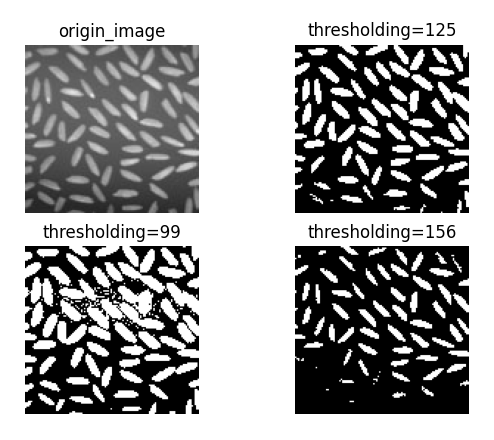
\includegraphics[width=0.31\linewidth,cframe=red!50!black 0.95mm]{14-1} &
 	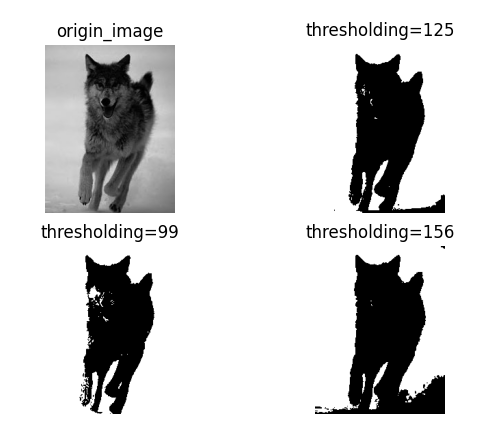
\includegraphics[width=0.31\linewidth,cframe=green!50!black 0.95mm]{14-2} &
    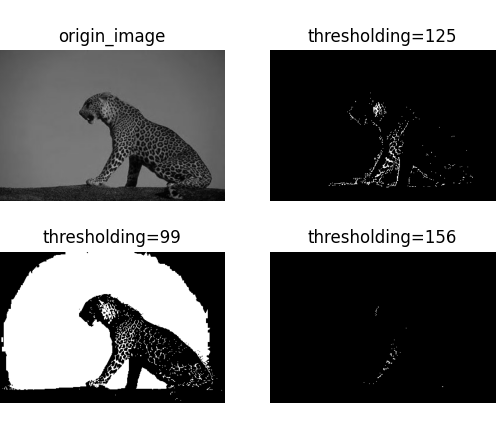
\includegraphics[width=0.313\linewidth,cframe=blue!50!black 0.95mm]{14-3} \vspace{-1mm}\\
%	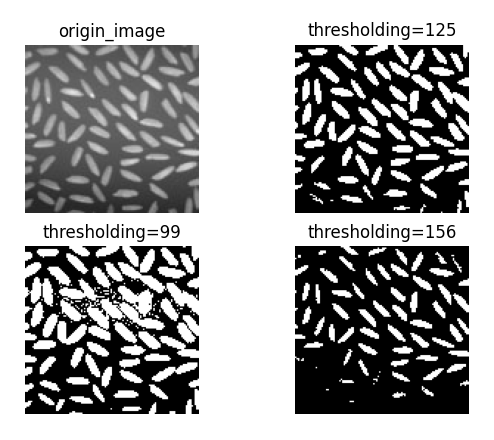
\includegraphics[width=0.31\linewidth]{14-1} &
% 	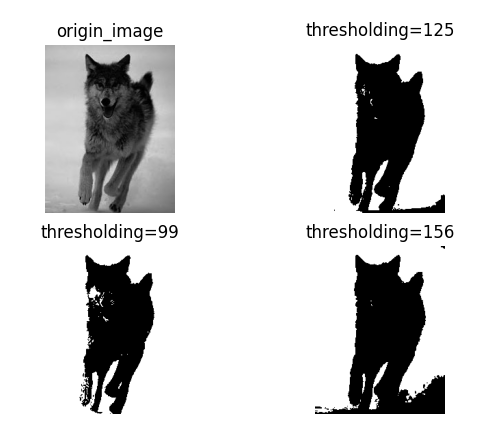
\includegraphics[width=0.31\linewidth]{14-2} &
%    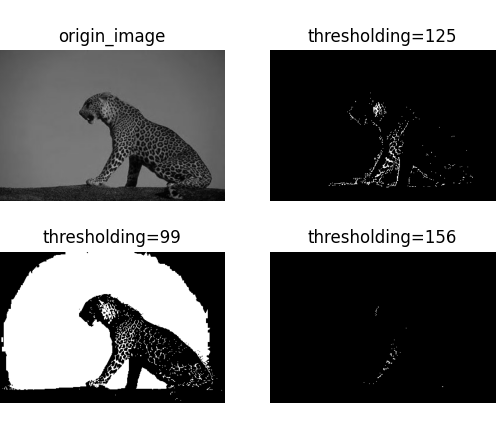
\includegraphics[width=0.32\linewidth]{14-3} \vspace{-1mm}\\
    \end{tabular}
	\captionof{figure}{\small 原始图像及三个不同阈值下的分割结果,三个阈值分别为125(右上)、99(左下)和156(右下)}
	\label{fig:random_thresholding}
	\end{center} 
\end{minipage}
}]

基于阈值的分割方法大多利用了图像的灰度直方图,它很好地反映了一幅图像中的灰度分布信息,是阈值选取的重要参考依据。在对直方图区域进行划分后,可以得到相应的直方图统计信息(目标/背景的先验概率、均值等),由此可以进一步求解不同的阈值选取准则函数。

图像分割旨在根据一定的准则将图像 $I$ 划分为不同区域的集合 $S$,集合 $S$ 满足下列条件:

\begin{enumerate}
	\item $\cup S_i = S$  
	\item $S_i \cap S_j=\emptyset,\;i \neq j$
	\item $\forall S_i,\; P(S_i)=true$
	\item $P(S_i\cup S_j)=false,\; i\neq j,\; S_i \; adjacent \; S_j$
\end{enumerate}
 
对于灰度图像而言,可以将其看作由目标(前景)和背景所构成,基于阈值的分割方法就是通过一个固定阈值将图像中的目标像素与背景像素进行分割,从而实现从图像中提取目标的目的。上述过程可以用下面的公式进行描述:

\begin{equation}
I'(x, y)=\left\{\begin{array}{l}
255, \;I(x, y)>\text{thresholding} \\[2em]
0, \;\quad I(x, y) \leq \text{thresholding}
\end{array}\right.
\vspace{0.5cm}
\end{equation}

其中,$\text{thresholding}$ 是设定的阈值,$x$ 与 $y$ 表示像素在图像中的坐标,$I(x, y)$ 为像素 $(x,y)$ 在原始图像中的灰度值,$I'(x, y)$ 为像素 $(x,y)$ 根据阈值分割后的二值图像对应的像素值。

阈值的选择对于基于阈值的分割方法而言至关重要。在理想条件下,目标和背景的灰度值具有明显的划分,可以将直方图的峰值之间的数值设置为阈值。但在实际应用中,由于各种环境因素的影响,目标和背景的灰度值界限并不易于区分,如 \textbf{图 \ref{fig:random_thresholding}} 所示,阈值设置过低时,背景中的噪声也会被划分到目标类别中,而当阈值设置过高时,目标中灰度值较低的部分被划入了背景部分。此外,对于不同的图像而言,相同的阈值也会取得不同的分割效果。因此,阈值的设置是基于阈值的分割方法的一大难题。图像分割阈值的设置常用方法包括:

\begin{itemize}
	\item 基于直方图形状:对去噪后的直方图的峰值、谷值和曲率等进行分析从而确定阈值
	\item 基于聚类:迭代找到阈值,并基于该阈值进行聚类
	\item 基于熵:选择一个使直方图信息量最大化的阈值
	\item 空间阈值(高阶统计):阈值的选择是基于空间邻域的高阶统计量
	\item 局部阈值:在每个邻域内利用局部统计信息寻找阈值
\end{itemize}

基于直方图的自适应阈值分割方法将图像的灰度直方图中的目标分量和背景分量分别参数化为模型(如高斯分布),然后在图像的灰度范围内迭代地设置不同的阈值,在当前阈值下,可以利用直方图的信息对模型中的未知参数进行估计(如高斯分布的均值、方差等),进而利用估计的参数对图像的整体灰度直方图进行“预测”。在同时具有“预测”分布和真实分布的情况下,就可以对不同阈值下“预测”的模型或分布进行评价,从而获得使拟合效果最好的阈值。

像的灰度直方图可以反映一幅图像中的灰度分布信息,能够为阈值的选取提供重要参考依据。基于直方图的自适应阈值分割方法,首先利用灰度直方图对图像的灰度分布进行统计。为了去除噪声的影响以及便于后续分布的拟合,要对直方图进行预处理,可以采用均值滤波或一维高斯滤波。为了对滤波处理后的灰度分布曲线进行拟合,同时将图像中的目标灰度值与背景灰度值进行区分,就需要分别建立符合目标和背景分量的直方图形状的参数模型,一般假设目标分量和背景分量的直方图形状近似服从高斯分布,而图像整体的灰度直方图形状即为由两个高斯分布组成的混合高斯分布。因此,在基于直方图的自适应阈值分割方法中,用下面两个高斯分布来分别代表目标和背景的分布:

\begin{equation}
f_o(g)=\frac{1}{\sqrt{2 \pi} \sigma_o} e^{-1 / 2\left(\frac{g-\mu_o}{\sigma_o}\right)^2}
\end{equation}

\begin{equation}
f_b(g)=\frac{1}{\sqrt{2 \pi} \sigma_b} e^{-1 / 2\left(\frac{g-\mu_b}{\sigma_b}\right)^2}
\vspace{0.5cm}
\end{equation}

其中,$f_o(g)$ 和 $f_b(g)$ 分别为目标和背景的分布函数,同时也表示灰度值为 $g$ 的像素占图像总体像素的百分比,$\mu_o$ 和 $\mu_b$ 分别为目标和背景的灰度均值,$sigma_o$ 和 $sigma_b$ 分别为目标和背景的标准差。

我们希望阈值可以将目标和背景的灰度分布进行分割,换句话来说,就是目标和背景的灰度可以分别分布在阈值的左右两侧。因此,我们可以假定一个阈值 $t$,然后对灰度图像直方图中阈值 $t$ 左右两侧的灰度信息进行统计计算,从而可以利用统计数据对 $f_o(g)$ 和 $f_b(g)$ 的均值及标准差进行估计,其估计方法如下所示:

\begin{equation}
\mu_o(t)=\sum_{g=0}^t f(g) g \quad \mu_b(t)=\sum_{g=t+1}^{\text {max }} f(g) g
\end{equation}

\begin{equation}
\sigma_o=\sum_{g=0}^t f(g) \left(g-\mu_o\right)  \quad \sigma_b=\sum_{g=t+1}^{\text {max }} f(g) \left(g-\mu_b\right)
\end{equation}

根据先验,我们可以得到一个像素落在目标或落在背景的概率分别为:

\begin{equation}
p_o(t)=\sum_t^{g=0} f(g)
\end{equation}

\begin{equation}
p_b(t)=1-p_o(t)
\vspace{0.5cm}
\end{equation}

对于假定的阈值 $t$,可以通过下面的公式对图像整体的灰度分布进行“预测”,并同样利用一维高斯滤波对估计的分布进行滤波处理:

\begin{equation}
P_t(g)=p_o f_0(g)+p_b f_b(g)
\vspace{0.5cm}
\end{equation}

最后,只需要在图像的灰度值变化范围内对潜在的阈值进行迭代,并通过计算 KL 散度来度量“预测”分布与真实分布之间的相似性,从而搜索到使得二者最相似的阈值即可,KL 散度的计算公式为:

\begin{equation}
K(t)=\sum_{g=0}^{\max } f(g) \log \left[\frac{f(g)}{P_t(g)}\right]
\vspace{0.5cm}
\end{equation}

对于复杂图像,在许多情况下对整幅图像用单一阈 值不能给出良好的分割结果。例如,由于照射光的 不均匀,虽然物体与背景始终有反差,但在图像的 某一部分物体和背景两者都比另一部分亮。克服这一缺点有如下一些方法:如果已知某个函数可以描述不均匀照射,就可以设法利用灰度级校正技术进行预处理(校正),然后采用单一阈值来分割;另外一种方法是把图像分成小块,并对每一块设 置局部阈值。但是,如果某块图像只含物体或只 含背景,那么对这块图像就找不到阈值。这时, 可以由附近的像块求得的局部阈值用内插法给该 像块指定一个阈值。

相比较人工设置阈值而言,基于直方图的自适应阈值分割方法可以更高效地寻找到可以较为准确地将灰度图像分割为目标和背景的阈值,计算简单、效率较高。但该方法也同样存在一定的问题,一方面是依赖于图像灰度值服从混合高斯分布的假设,但真实的图像分布并不一定是服从高斯分布的,一旦这个假设不成立,那么该方法的准确性也会受到一定的影响;另一方面该方法只考虑了像素的灰度值,而一般不考虑图像的空间特征,使其对噪声比较敏感,鲁棒性不高。这也是传统方法普遍存在的局限性——高度依赖于人工设计的特征。另一个问题就是传统方法很难给出分割结果的语义信息,更别说不同实例的信息,而语义对于图像理解来说可能是非常重要的。

随着深度学习技术的快速发展,上述问题得到了一定的解决,尤其是在图像的语义分割和实例分割方面。图像分割研究像素分组问题。像素分组的不同语义(例如类别或实例)导致了不同类型的分割任务,例如全景、实例或语义分割。虽然这些任务仅在语义上有所不同,但当前的方法为每个任务开发专门的结构。基于全卷积网络(FCN)的逐像素分类体系结构用于语义分割,而预测一组二进制掩码的掩码分类结构则主导了实例分割。尽管这种专门的结构改进了每个单独的任务,但它们缺乏推广到其他任务的灵活性。例如,基于FCN的结构在实例分割方面存在困难。因此,重复的研究和硬件优化工作花费在每个针对任务的专用结构。

\begin{figure}[!tbp]
	\centering
	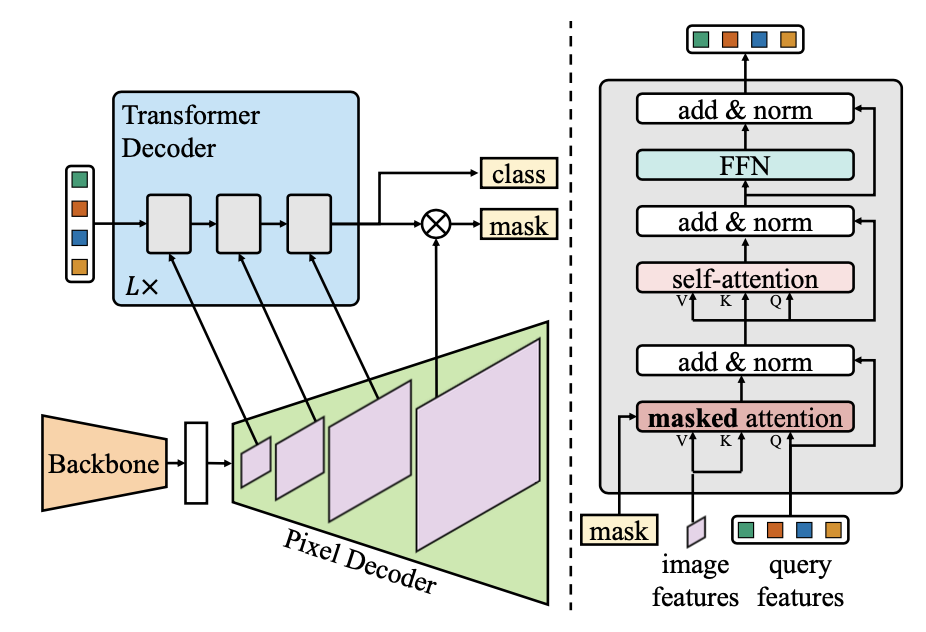
\includegraphics[width=\linewidth]{15.png}
	\caption{Mask2Former 网络结构图}
	\label{fig:fig15}
\end{figure}

为了解决这种分割问题,最近的工作试图设计通用架构,能够用相同的架构处理所有分割任务(即通用图像分割)。这些结构通常基于端到端集预测目标(例如,DETR),并在不修改结构、损失或训练过程的情况下成功地处理多个任务。尽管具有相同的体系结构,但通用结构仍然针对不同的任务和数据集分别进行训练。尽管现有的通用结构足够灵活,可以处理任何细分任务,但在实践中,它们的性能落后于最好的专用结构。除了性能较差之外,通用结构也更难训练。他们通常需要更先进的硬件和更长的训练时间。性能和训练效率问题都阻碍了通用结构的部署。

Masked attention Mask Transformer(Mask2Former) \cite{DBLP:conf/cvpr/ChengMSKG22}作为通用的图像分割体系结构可以在不同的分割任务中都优于专用的结构,同时在每个任务上都很容易训练。如 \textbf{图 \ref{fig:fig15}} 所示,模型由从图像中提取低分辨率特征的主干网络;从主干输出中逐渐向上采样低分辨率特征,以生成高分辨率的每像素嵌入的像素解码器;对图像特征进行操作以处理对象查询的Transformer解码器三部分组成。

 K-Net \cite{zhang2021k}是一种通过一组可学习的核来统一图像分割(语义分割、实例分割)的方法。这些来自 K-Net 的可学习的核可以在视频帧中自然地关联相同的实例。基于 K-Net,Video K-Net \cite{li2022video}通过简单的基于核的外观建模和跨时间内核交互,学会了同时分割和跟踪视频中的``things''和``stuff''(语义分割和实例分割),实现了简单、强大、统一的端到端视频全景分割框架。在Citscapes VPS 和 KITTI-STEP 上实现了最先进的视频全景分割结果。可以看到,无论是在图像分割还是在视频分割领域,通用的分割框架是当下的一个研究热点。